\documentclass[12pt,letterpaper]{amsbook}

%%%%%%%%%%%%
% Includes %
%%%%%%%%%%%%
\usepackage[utf8]{inputenc}
\usepackage[margin=1 in]{geometry}
\usepackage{parskip}
\usepackage{graphicx}
\usepackage{amsmath}
\usepackage{amsthm}
\usepackage{amsfonts} 
\usepackage[ruled,vlined]{algorithm2e}
\usepackage[justification=centering]{caption}
\usepackage[hidelinks]{hyperref}

% Formatting
\renewcommand{\baselinestretch}{1.25}

% Theorems and other necessary structures
\theoremstyle{definition}
\newtheorem{definition}{Definition}[section] % Definition
\newtheorem{theorem}{Theorem}[section] % Big result
\newtheorem{corollary}{Corollary}[theorem] % Follows from a theorem
\newtheorem{lemma}[theorem]{Lemma} % Minor result

% New commands
\newcommand{\R}{\mathbb{R}} % Real numbers
\newcommand{\N}{\mathbb{N}} % Natural numbers
\newcommand{\Z}{\mathbb{Z}} % Integral numbers

% Title information
\title{Compilers}
\author{2018A7PS0193P}

\begin{document}

\maketitle

\chapter{Process of Translation}

The process of compilers converting from source code (the high level language) to target code (the machine language) is known as translation.  It consists of many steps, which are described below.

\section{Lexical Analysis}

Lexical analysis follows the following steps:

\begin{enumerate}
  \item Identify the valid set of characters in the language
  \item Break the sequence of characters into appropriate words or tokens (keywords, numbers, operators, etc.)
  \item Find out whether these tokens are valid or not.
\end{enumerate}

The key goal of the lexical analyzer is to break a sentence into a series of words/tokens. These breaks are generally done via certain separators. The tokens are recognized via some rules encoded into a Finite State Machine.

During the lexical phase, we may experience the following lexical errors:

\begin{itemize}
  \item Occurrence of illegal characters
  \item Exceeding the length of identifier
\end{itemize}

The output of the lexical analyzer will be a sequence of tokens and their ``type'', which signifies whether it is a identifier, operator, etc.

\section{Syntax Analysis}

The syntax analysis takes the sequence of tokens as an input, and generates a parse tree. In case the syntax is not correct according to the grammar rules, it flags a syntactical error. This is modelled using Context Free Grammars that will be recognized using PDAs or Table Driven processes.

\section{Semantic Analysis}

Semantic analysis takes the parse tree as an input, and outputs a disambiguated parse tree. It performs the following:

\begin{itemize}
  \item Check Semantics
  \item Error reporting (types, etc.)
  \item Disambiguate overloaded operators (meaning of operators depends on operands)
  \item Type coercion (type casting)
  \item Uniqueness checking (redeclaration of variables)
\end{itemize}

As such, the disambiguated parse tree gives us an unambiguous representation of the parse tree.

The phases mentioned till now comprise the \textbf{front end} of the compiler, where the source code is handled. After this, the compiler works on generating the target code.

\section{Code optimization}

This is an optional phase that modifies the programs to run faster and consume less resources like memory, registers, etc. However, it will not change the representation of the program.

Some examples of machine independent code optimization done is:

\begin{itemize}
  \item \textbf{Common sub-expression elimination:} The compiler searches for instances of identical expressions and analyzes whether it is worthwhile to replace them with a single variable holding the computer value.
  \item \textbf{Copy Propagation:} The compiler replaces the occurrences of targets of direct assignments with their value. For instance, if we had the code \texttt{y=x; z = 3+y;}, copy propagation would yield \texttt{z=3+x;}
  \item \textbf{Dead code elimination:} The compiler removes code which does not affect the program results, including unreachable code and unused variables.
  \item \textbf{Code Motion:} The compiler moves statements and expressions out of the body of a loop if they are loop-invariant, i.e., doing so does not affect program semantics.
  \item \textbf{Strength Reduction:} The compiler replaces expensive operations with equivalent but less expensive operations.
  \item \textbf{Constant Folding:} The compiler recognizes and evaluates constant expressions at compile time instead of runtime.
\end{itemize}

\section{Code Generation}

This is the process of mapping from source level abstractions (identifiers, values, etc) to target machine abstractions (registors, memory, etc.). This is a two step process - initially, intermediate code gets generated from the disambiguated parse tree, which is used to generate the final machine code.

During code generation, we have to do the following:

\begin{itemize}
  \item Map identifiers to locations (memory or registers)
  \item Map source code operators to opcodes or sequences of opcodes.
  \item Transform conditionals and iterations to a test/jump or compare instructions
  \item We use layout parameter passing protocols - the locations for parameters, return values, etc.
\end{itemize}

\section{Post Translation Optimizations}

Unlike in the code optimization phase where we perform machine independent code optimizations, this does machine-dependent code optimizations. This is an optional phase as well, where we may remove unneeded operations or rearrange to prevent hazards. It is a flexible phase, and may occur at any time in the back-end of the compiler.

\section{Symbol Table}

The symbol table contains information required about the source program identifiers during compilation, including:

\begin{itemize}
  \item Category of variable
  \item Data type
  \item Quantity stored in structure
  \item Scope information
  \item Address in Memory
\end{itemize}

The symbol table must be present in every phase of the compiler, and is used in all the phases to get information about the identifiers.

\section{Advantages and Disadvantages of Compilers}

The advantages of compilers are:

\begin{itemize}
  \item Highly modular in nature
  \item It is retargetable. This means that if there is a single language and multiple machines, then we can use the same front end.
  \item Source code and machine independent optimizations are possible.
\end{itemize}

The limitations of the compiler are:

\begin{itemize}
  \item Design of programming languages has a huge effect on the performance of compilers.
  \item Lots of work is repeatable. For $S$ languages and $M$ machines, $S\cdot M$ compilers are needed. This is known as the $S*M$ problem of compilers.
\end{itemize}

The $S*M$ problem is generally solved by introducing some common intermediate language, called the \textbf{Universal Intermediate Language Generator}. Some common machine independent intermediate code generation techniques are:

\begin{itemize}
  \item Postfix Notation
  \item Three Address code
  \item Syntax tree
  \item Directed Acyclic Graph
\end{itemize}


\chapter{Lexical Analysis}

\section{Functions of the Lexical Analyzer}

The lexical analyzer performs the following functions:

\begin{itemize}
  \item Take high level language as input and output a sequence of tokens
  \item It generally cleans the code, by stripping off blanks, tabs newlines and comments.
  \item Keeps track of the line numbers for associated error messages
\end{itemize}

The lexical analyzer is modelled using regular expressions. As such, it's implementation is done with a DFA. An example of one rule is $L \cdot (L+D)^*$, where $L$ refers to a letter and $D$ refers to a digit.

\begin{definition}
  A token is a string of characters which logically belong together, e.g. keywords, number, identifiers, etc.
\end{definition}

\begin{definition}
  A pattern is the set of strings for which the same token is produced.
\end{definition}

\begin{definition}
  A lexeme is a sequence of characters matched by a pattern to form the corresponding token.
\end{definition}

Now that we understand the definitions, we can see what the lexical analyzer actually does - it transforms strings to the token and passes the lexeme as it's corresponding attribute. For instance, the integer 43 would become \texttt{<num,43>}.

\section{Working of the Lexical Analyzer}

The lexical analyzer reads the character one by one from the source code into the lexeme. When it reaches a separator, it assigns a token to the lexeme based on certain rules, and continues to read the characters once more.

However, reading the lexemes character by character is slow, and involves many IO operations. This is done from a buffer instead of directly from the file. Moreover, the prefix of a lexeme is often not enough to determine the token - think of the lexemes \texttt{=} and \texttt{==}. We instead use a lookahead pointer to determine the appropriate token for a lexeme, and then push back the characters that we do not need in the current lexeme.

\section{Symbol Table and the Lexical Analyzer}

The lexical analyzer also interfaces with the symbol table. When the lexical analyzer discovers a lexeme constituting an identifier, it enters that lexeme to the symbol table. Sometimes, information regarding the token of a particular lexeme may also be store in the symbol table. As such, the symbol table must implement the following operations:

\begin{enumerate}
  \item \texttt{insert(s,t)} : Save lexeme \texttt{s} and token \texttt{t} and return pointer.
  \item \texttt{lookup(s)} : return the index of entry for lexeme \texttt{s} or \texttt{`0'} if \texttt{s} is not found.
\end{enumerate}

To make the symbol table space efficient, we save lexemes in some separate memory, and instead store pointers to the lexemes in the symbol table.

The rule for identifying an identifier and a keyword is generally the same. To be able to tokenize the identifiers and keywords separately, we initialize the symbol table with the list of keywords, say, by calling \texttt{insert("if",keyword)}.

\section{Challenges in Development of Lexical Analyzer}

\begin{itemize}
  \item \textbf{Free vs Fixed Lexemes} : A language could specify that lexemes must be in a free or a fixed format. For instance, in a free format, code could look like this.
    \begin{verbatim}
    flag = flag
    * 6;
    \end{verbatim}
    But in the case of fixed format, this must be entirely in one line. An example of a fixed format language is Python, while a free format language is C.
  \item \textbf{Whitespaces} : How do we deal with whitespaces? Some languages ignore whitespaces until a separator is reached (or interpret contextually), while some languages consider the whitespaces as separators themselves. The former is much more complicated to implement than the latter.
  \item \textbf{Maximal Munch} : The principle of maximal munch directs the lexical analyzer to consume as much available input as possible while creating a construct. This allows us to deal with lexemes like \texttt{iff}, and correctly assign it as a identifier rather than the keyword \texttt{if}.
\end{itemize}

\section{Techniques for specifying tokens} 

\begin{definition}
  Consider $R_i$ is a regular expression and $N_i$ is a unique name, then a regular definition is a series of definitions of the following form 
  \[N_1 \rightarrow R_1 \]
  \[N_2 \rightarrow R_2 \]
  \[...\]
  \[N_n \rightarrow R_n \]
  where each $R_i$ is a regular expression over $\sum \cup \{N_1,N_2,...N_n\}$.
\end{definition}

Hence, by assigning a special name $N_i$ to the regular expression $R_i$, we are in effect defining macros, that remove redundancy in later parts.

The following is an example regular definition for identifiers:

\[\text{Alphabet} \rightarrow A|B|C|...Z|a|b|c|...|z\]
\[\text{Digit} \rightarrow 0|1|2|...|9\]
\[\text{Identifier} \rightarrow \text{Alphabet}(\text{Alphabet} | \text{Digit})^*\]

This too comes with its own challenges. Regular expressions often fail when identifying the appropriate token, and may pass the invalid tokens to the subsequent translation phases of the compiler (how?). They are only language specifications. Tokenization is a implementation problem.

Tokenization can be done via the following steps:

\begin{enumerate}
  \item Construct regular expressions for lexemes of each token
  \item Construct $R$ matching all lexemes of tokens, so $R = R_1+R_2+...$, in some well defined precedence order.
  \item Consider the input stream to be $S=s_1s_2...s_n$. For $i \in [1,n]$, verify whether $s_1...s_i \in L(R)$.
  \item If $s_1...s_i \in L(R) \implies s_1..s_i \in L(R_x)$ for some $x$. We choose the smallest $x$ to be the class of $s_1..s_i$. 
  \item Discard the tokenized input and go back to step 3.
\end{enumerate}

The procedure gives preference to tokens specified earlier using regular expressions. If $s_1..s_i \in L(R)$ and $s_1...s_j \in L(R)$, we choose the longest prefix, in accordance with the principle of maximal munch.

To implement our regular definitions and recognize tokens, we use \textbf{transition diagrams}. They are shown diagrammatically in the same way as Finite Automata. Transitions can be labelled with a symbol, a group of symbols, or regular definitions. A few states may be \textbf{retracting states} that indicates that the lexeme does not include the symbol that can bring us to the accepting state.

Sometimes, we may want to push back extra characters into the token stream (think of \texttt{>} and \texttt{>=}, we may want to push back the extra character read if the token is \texttt{>}). We mark those states with a \texttt{*}, to show that we must push back extra characters.

Let us consider the example of hexadecimal and octal constant. The regular definition would be:

\[hex \rightarrow 0|1|2|...|9|A|B|C|...F\]
\[oct \rightarrow 0|1|2|...|7\]
\[Qualifier \rightarrow u|U|l|L\]
\[OctalConstant\rightarrow 0 oct^+(Qualifier|\epsilon)\]
\[HexadecimalConstant\rightarrow 0(x|X)hex^+(Qualifier|\epsilon)\]

The transition diagram for the given regular definition is given in Fig 1.

\begin{figure}[htpb]
  \centering
  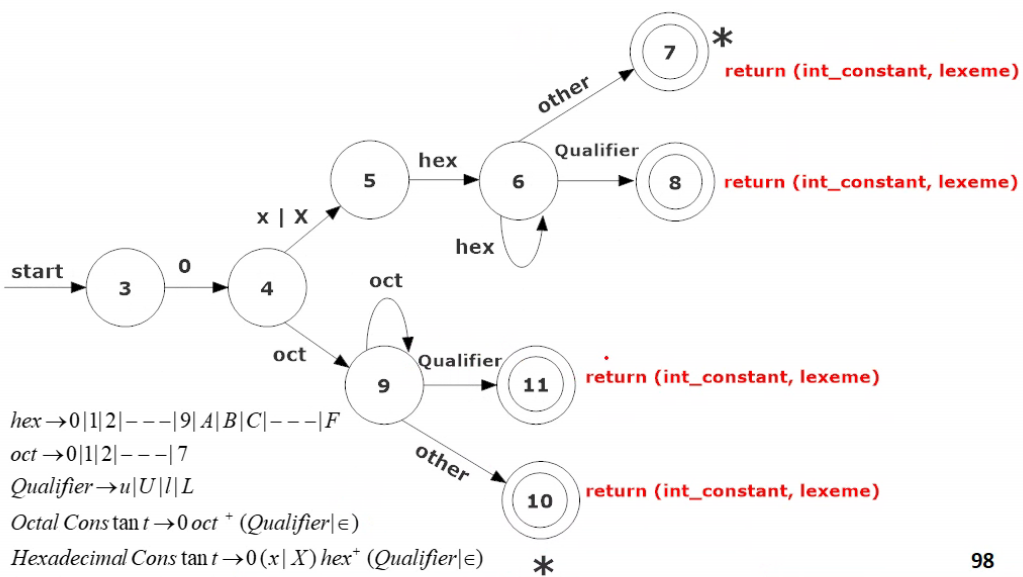
\includegraphics[width=0.8\linewidth]{./assets/hex_oct_trans_diag.png}
  \caption{Transition diagram for the Hex and Octal constants}%
  \label{fig:}
\end{figure}

The retracting states are not given. If we get a ``bad character'', we should report it as a lexical error.

Let us consider another example of a generalized expression for unsigned numbers. The regular definition is:

\[Digit \rightarrow 0|1|2|...|9\]
\[Digits \rightarrow Digit^+\]
\[Fraction \rightarrow .Digits|\epsilon\]
\[Exponent \rightarrow (E(+|-|\epsilon)Digits)|\epsilon\]
\[Number \rightarrow Digits \cdot Fraction \cdot Exponent\]

The resulting transition diagram from this is in Fig 2.

\begin{figure}[htpb]
  \centering
  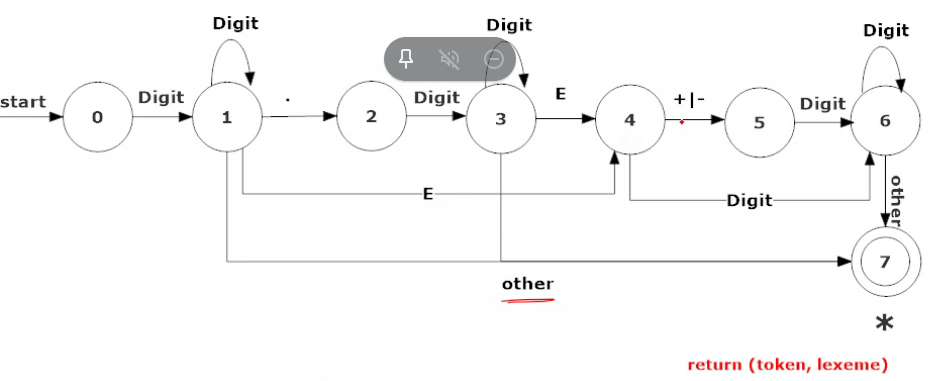
\includegraphics[width=0.8\linewidth]{./assets/unsigned_num_trans_diag.png}
  \caption{Transition Diagram for Unsigned Numbers}%
  \label{fig:}
\end{figure}

The issue here is this often introduces a lot of complexity. Instead, we may add split this into multiple transition diagrams, to improve implementation complexity. This also is seen empirically to give better speeds. These multiple transition diagrams can be appropriately combined to generate a lexical analyzer.

The matching process should always start with some transition diagram. If failure occurs in one transition diagram, we retract the forward pointer to the start state, and activate the next transition diagram. If there is failure in all the transition diagrams, we throw a lexical error.

\chapter{Syntax Analysis}

\section{Grammar Rules}

Regular definitions are not enough for syntax analysis, since languages are generally not regular. Instead, we use Context Free Grammars to model our language, given by $G = \{T,N,P,S\}$, where

\begin{itemize}
  \item $T$ is the set of tokens (or terminals)
  \item $N$ is the set of non-terminals
  \item $P$ is the set of production rules
  \item $S$ is the start symbol.
\end{itemize}

However, just creating the CFG is not the end of our problems - we must choose a method of derivation (left vs right), choose the right non-terminal to expand, choose the right production rule and maintain some precedence order.

When we replace the leftmost non-terminal in any sentential form of the grammar, it is called \textbf{leftmost derivation}. Choosing the rightmost non-terminal makes it \textbf{rightmost derivation}. If a grammar generates more than one leftmost/rightmost derivation of a string, it is said to be \textbf{ambiguous}.

The end goal of our syntax analysis is to create the \textbf{parse tree} - where the root is a start symbol, internal nodes are non-terminals and leaf nodes are labelled by tokens. An ambiguous grammar can have more than one parse tree.

Unfortunately, no well defined algorithm exists to remove ambiguity in a grammar. However, we can manually convert any ambiguous grammar into an unambiguous grammar. We can do this by enforcing associativity and precedence rules. This is pretty well covered in PPL and TOC.

Remember that right associativity is created via right recursion ($N \rightarrow \alpha N$) and left associativity is created via left recursion ($N \rightarrow N \alpha$)

In programming languages, ambiguity can come in many forms. For instance, consider the sentence \texttt{if A then if B then C1 else C2}.  This could be:

\begin{verbatim}
if A then 
{
  if B then
    C1
  else
    C2
}
\end{verbatim}

or:

\begin{verbatim}
if A then 
{
  if B then
    C1
}
else
  C2
\end{verbatim}

Since there is ambiguity in its meaning, we must resolve it. One way to do this is to relate an \texttt{if} with the closest unrelated \texttt{else} (the second interpretation). Another way is to match each \texttt{else} with the closest previous \texttt{then}(the first interpretation). The unambiguous grammar would then be:

\[stmt \rightarrow matchedstmt | unmatchedstmt\]
\[matchedstmt \rightarrow \text{if }exp \text{ then } matchedstmt \text{ else } matchedstmt | others\]
\[unmatchedstmt \rightarrow \text{if }exp \text{ then } stmt | \text{if }exp \text{ then } matchedstmt \text{ else } unmatchedstmt\]

\section{Parsing}

Resolving ambiguity is the problem of the language specification, not of the syntax analysis. Parsing is the job of implementation. We can do this in two ways:

\begin{itemize}
  \item \textbf{Top down parsing:} Construction of the parse tree starting from the root node (start symbol) and proceeds towards the leaves (terminals).
  \item \textbf{Bottom up parsing:} Construction of the parse tree starts from the terminal nodes and builds up towards the root node(start symbol).
\end{itemize}

\section{Top Down Parsing}

In top down parsing, we repeat the following two steps:

\begin{enumerate}
  \item At a node labelled with non-terminal $A$, select one of the productions of $A$ and construct the children nodes.
  \item Find the next node at which the subtree is to be constructed.
\end{enumerate}

To choose the production rule, as in step 1, backtracking must be done. We try every production rule that we can apply and see which one works. The parser must be intelligent enough to choose the production rule to apply based on the token being pointed to by the pointer.

\section{First Set}

If we could determine the first character of the string produced when a production rule is applied, we could compare it to the current token and choose the production rule correctly. For this, we use a concept called the First Set.

The \textbf{First set}, denoted by \texttt{FIRST(X)} for a grammar symbol $X$ is the set of tokens that begin the strings derivable form $X$. If there is a production rule:
\[A \rightarrow \alpha\]
then First($A$) is the set of tokens that appear as the first token in strings generated from $\alpha$.

To compute FIRST($X$), we use the following rules:

\begin{enumerate}
  \item If $X$ is a terminal, then FIRST($X$) $= \{X\}$
  \item If $X$ is a non terminal and $X \rightarrow Y_1Y_2...Y_k$ is a production for $k \geq 1$, then place $a$ in First($X$) if for some $i$, $a$ is in First($Y_i$) and $\epsilon$ is in all of First($Y_j)$ for $j < i$. If $\epsilon$ is in all $Y_i$, then add $\epsilon$ to First($X$).
  \item If $X \rightarrow \epsilon$, then add $\epsilon$ to First($X$).
\end{enumerate}

Consider the following example:
\[S \rightarrow ABCDE\]
\[A \rightarrow a|\epsilon\]
\[B \rightarrow b|\epsilon\]
\[C \rightarrow c\]
\[D \rightarrow d|\epsilon\]
\[E \rightarrow e|\epsilon\]
Then, the first sets are as following:
\begin{itemize}
  \item First($S$) = $\{a,b,c\}$
  \item First($A$) = $\{a,\epsilon\}$
  \item First($B$) = $\{b,\epsilon\}$
  \item First($C$) = $\{c\}$
  \item First($D$) = $\{d,\epsilon\}$
  \item First($E$) = $\{e,\epsilon\}$
\end{itemize}

\section{Recursive Descent Parser}

Let us look at our first parser - the \textbf{recursive descent parser}. RDP is a top down method of syntax analysis in which a set of recursive procedures are executed to parse the stream of tokens. A procedure is associated with each non-terminal of the grammar. The procedure generally implements one of the production rules of the grammar.

In each procedure, we perform a match operation on hitting any token on the RHS of the grammar with the current token in the input that needs to be parsed. For example, if we have the string $aba$ and the rule $S \rightarrow abB$, it will match the tokens $a$ in both the RHS and the string, and move on to the next token. If there is no match, we throw a syntax error.

This approach, of course, has it's own limitations. Consider a grammar with two productions:
\[X \rightarrow \gamma_1\]
\[X \rightarrow \gamma_2\]
Suppose First($\gamma_1$) $\cap$ First($\gamma_2$) $\neq \phi$, and that $a$ is the common terminal symbol. In cases like this, we need to perform backtracking to choose the right production rule. However, RDP does not support backtracking right now. To support it, all productions should be tried in some order. Failure for some productions implies we need to try remaining productions. We would report an error only when there are no other rules.

Moreover, a recursive descent parser may loop forever on productions of the form:
\[A \rightarrow A \alpha_1|A \alpha_2 | ... | A \alpha_n | \beta_1 | ... | \beta_m\]
This is known as left recursion. We can remove it from the grammar by rewriting the rule as:
\[A \rightarrow \beta_1 A' | \beta_2 A' | ... | \beta_m A'\]
\[A' \rightarrow \alpha_1 A'| \alpha_2 A' | ... | \epsilon\]
Left recursion can be hidden as well, where expanding production rules in some order could lead to left recursion. This is called hidden left recursion, and we must handle it in the same way as we did left recursion.

Left factoring is the process of removing the common left factor that appears in two productions of the same non-terminal. An example of a rule to remove is:
\[A \rightarrow \alpha \beta_1|\alpha \beta_2 | ... | \alpha \beta_n\]
We can remove the left factoring and get:
\[A \rightarrow \alpha A'\]
\[A' \rightarrow \beta_1|\beta_2| ... | \beta_n\]
In the initial form, the parser would be confused about which production rule to try. With the second case, we can kick the can down the road, and use a (hopefully) single lookahead pointer to decide what to do with $A'$.

\section{Follow Set}

Consider the following grammar:
\[A \rightarrow aBb\]
\[B \rightarrow c | \epsilon\]
And suppose we want to parse an input string ``ab''. How would the parser know to use $\epsilon$ for $B$? To do this we use the \textbf{follow set}.

Follow($X$) for a non terminal $X$ is the set of symbols that might follow the derivation of $X$ in an input stream. The follow of the start symbol $S$ is \{\$\}. The follow set can never be $\epsilon$, since if it ends with an epsilon, the follow would be the ending symbol of the string -  the \$. The steps to compute the follow set is:

\begin{itemize}
  \item Always include \$ in Follow($S$).
  \item If there is a production rule $A \rightarrow \alpha B \beta$, where $B$ is a non terminal, then Follow($B$)  = First($\beta$).
  \item If there is a production rule $A \rightarrow \alpha B \beta$, where $B$ is a non terminal, and First($\beta$) contains $\epsilon$, then everything in Follow($A$) is in Follow($B$).
  \item If there is a production rule $A \rightarrow \alpha B$, then Follow($B$) = Follow($A$).
\end{itemize}

\section{Predictive Parsing}

Now that we have talked about all the issues that can face RDP, let us look at a new parser - \textbf{predictive parsing}. This is a non recursive top down parsing method, which recognizes LL(1) languages. LL languages are those that can be parsed by an LL parser, which parses the input from left to right, and constructs a leftmost derivation. The 1 means that we use one input symbol of lookahead to make parsing action decisions. The predictive parser makes use of a parse table and a stack to process the input token stream.

The parse table is a two dimensional array $M[X,a]$ where $X$ is a non terminal and $a$ is a terminal. This parse table tells the parser which production rule to use when we have a non-terminal $X$ on top of the stack and the lookahead pointer points to $a$. This parse table is generated by using the First and Follow set of every non-terminal in the grammar.

To construct the parse table, we do the following steps for each production rule $A \rightarrow \alpha$:

\begin{enumerate}
  \item For each terminal $a$ in First($\alpha$), $M[A,a] = A \rightarrow \alpha$
  \item If $\epsilon$ is in First ($\alpha$), $M[A,b] = A \rightarrow \alpha$ for each terminal $b$ in Follow(A).
  \item If $\epsilon$ is in First($\alpha$), and \$ is in Follow($A$), $M[A,\$] = A \rightarrow \alpha$.
\end{enumerate}

Now we can finally see the algorithm for predictive parsing. Consider that \$ is a special token at the bottom of the stack and also terminates the input string. Assume that initially, the predictive parser has $X$ symbol on top of the stack and $a$ is the current input symbol. Then, the predictive parser does the following:

\begin{itemize}
  \item If $X=a=\$$, then stop.
  \item If $X = a \neq \$$, then pop $X$ and increment the lookahead pointer.
  \item If $X$ is a non terminal, then
    \begin{itemize}
      \item If $M[X,a] = X \rightarrow PQR$, then pop $X$ and push $R,Q,P$.
      \item Else, throw an error
    \end{itemize}
\end{itemize}

Predictive parsing needs a LL(1) Grammar. A grammar is LL(1) if the constructed parse table has no multiple entries. If it does have multiple entries of in the same cell, it cannot be LL(1), and cannot be parsed using predictive parsing.

Another way to tell if a grammar is LL(1) is to consider rules of the type:
\[A \rightarrow \alpha_1 | \alpha_2 | \cdots | \alpha_n\]
All rules of this type must be such that $\bigcap_{i=1}^n First(\alpha_i) = \phi$ and rules of the type:
\[A \rightarrow \alpha | \epsilon\]
must be such that $First(\alpha) \cap Follow(A) = \phi$.

\section{Error Recovery}

The compiler must recover from errors and identify as many errors as possible. For this, the most frequently used error technique is \textbf{panic mode}.

In panic mode, when an error is encountered anywhere in the statement, the rest of the statement is ignored by not processing the input from erroneous input to delimiters. This mode prevents the parser from developing infinite loops and is considered as the easiest way for recovery of the errors.

The error is detected when an entry in the parse table is empty. We then skip over symbols in the input until a token in a selected set of \textbf{synchronizing tokens} appears. If the error occurs for the parse table entry $M[A,a]$, we place the symbols in Follow($A$) in a synchronizing set in the parse table. So, we skip tokens until an element in the synchronizing set appears, then pop $A$ and continue parsing from that token.

\section{Bottom Up Parsing and Shift-Reduce Parsing}

In bottom up parsing, we design a parse tree for an input string starting from the leaf nodes and going towards the root. This is equivalent to finding a series of steps to reduce a string $w$ of input to the start symbol of the grammar by tracing out the rightmost derivations of $w$ in reverse.

Bottom up parsing is done via \textbf{shift reduce parsing}. Shift reduce parsing splits the string into two parts,  separated by a special character `.'. The left part is a string of terminals and non terminals (on the stack), and the right part is a string of terminals (rest of the input string). Initially, we assume the input to be $.w$ . The parser does one of two operations:

\begin{itemize}
  \item \textbf{Shift:} It moves terminal symbol from the right part of the string to the left part of the string. If string before the shift if $\alpha . pqr$, then the string after shift is $\alpha p . q r$. This is equivalent to pushing a terminal onto the stack.
  \item \textbf{Reduce:} It occurs immediately on the left of `.' and identifies a string name as RHS of a production and replaces it by the LHS. If string before reduce action is $\alpha \beta . p q r$ and $A \rightarrow \beta$ is a production then string after reduction is $\alpha A . pqr$. This is equivalent to popping the RHS of the production, and pushing the LHS onto the stack.
\end{itemize}

Bottom up parsing is capable of handling left recursive grammars.

A string that matches the RHS of a production and whose replacement gives a step in the reverse of right most derivation is called a \textbf{handle}. Our goal is to always reduce the handle and not just any RHS. Hence the shift reduce parser must be capable of detecting these handles.

A shift reduce parser could also find a \textbf{conflict}. A shift-reduce conflict is when both a shift and a reduce operation are valid. A reduce-reduce conflict is when reduction can be done by more than one production rule.

\section{The LR(0) Parser}

Now let us look at our first bottom up parser, the LR(0) parser. LR parsers are those that read from left to right, producing a rightmost derivation in reverse. LR(0) uses 0 tokens of lookahead to make it's predictions. Before we discuss the exact algorithm we must understand some concepts.

\subsection{Augmentation of Grammar}

If $G$ is a grammar with a start symbol $S$, the augmented grammar $G'$ which has a new start symbol $S'$ and a additional production:
\[S' \rightarrow S\]
When the parser reduces by this new rule, it will stop immediately in the accept state.

\subsection{LR(0) Items}

An LR(0) item of a grammar is a production of $G$ with a special symbol `.' at some position on the RHS. So, the production $A \rightarrow XYZ$ gives four LR(0) items:
\[A \rightarrow .XYZ\]
\[A \rightarrow X.YZ\]
\[A \rightarrow XY.Z\]
\[A \rightarrow XYZ.\]
Each item indicates how much of a production has been seen at a point in the process of parsing. For instance, the second rule indicates that we have seen an input string derivable from $X$ and hope to see a string derivable from $YZ$ on the next input.

\subsection{Closure}

Let $I$ be a set of items for a grammar $G$. Then the Closure($I$) is a set constructed as follows:

\begin{itemize}
  \item Every item $I$ is in closure($I$)
  \item If $A \rightarrow \alpha . B \beta$ is in closure ($I$) and $B \rightarrow \gamma$ is a production then $B \rightarrow .\gamma$ is in closure($I$).
\end{itemize}

\subsection{Goto}

The Goto operation, defined by Goto($I,X$), where $I$ is a set of items and $X$ is a grammar symbol, is closure of set of items $A \rightarrow \alpha X. \beta$ such that $A \rightarrow \alpha . X \beta$ is in $I$. If $I$ is a set of items for some valid prefix $\alpha$, then Goto($I,X$) is set of valid items for prefix $\alpha X$. 

\subsection{LR(0) Automaton}

The goal of the LR(0) parser is to create a LR(0) automaton, also called the Goto graph. The states of the automaton are the sets of items of the LR(0) collection, and the transitions are given by the Goto function. The start state of this automaton is Closure($\{S' \rightarrow .S\}$). All the states are accepting states.

This automaton helps us with shift-reduce decisions. Suppose that the string $\gamma$ of grammar symbols takes the LR(0) automaton from the start state 0 to some state $j$. Then, shift on the next input symbol $a$ if state $j$ has a transition on $a$. Otherwise, we reduce; the items in state $j$ tell us which production to use.

\subsection{Parsing Table}

This LR(0) automaton is encoded in the \textbf{parsing table}. It consists of two parts - a parsing action function ``Action'' and a goto function ``Goto''.

The Action function takes as arguments a state $i$ and a terminal $a$ (or \$, the input end marker). The value of Action($i,a$) can have one of four forms:
\begin{enumerate}
  \item Shift $j$, where $j$ is a state. The action taken by the parser effectively shifts input $a$ onto the stack, but uses state $j$ to represent $a$. This is denoted by $sj$.
  \item Reduce $A \rightarrow \beta$. The action of the parser effectively reduces $\beta$ on the top of the stack to head $A$. This is denoted by $rj$, where $j$ is the number of the production.
  \item Accept the input and finish parsing. This is denoted by acc.
  \item Error. This is denoted by a blank cell.
\end{enumerate}

The Goto function maps a state $i$ and a non terminal $A$ to state $j$ if Goto($I_i,A$) = $I_j$

\subsection{Is this Grammar LR(0)?} 

A grammar is LR(0) if its LR(0) parsing table does not contain multiple defined entries. Another way is to check if it has any shift-reduce/reduce-reduce conflicts.

\subsection{Contents of LR Parser}

The configuration of a LR parser is defined by the 2-tuple (Stack Contents, Remaining Input). Hence, the initial configuration would be $(S_0,a_0a_1a_2...a_n\$)$

\subsection{Example}

Let us consider the grammar
\[S \rightarrow AA\]
\[A \rightarrow aA|b\]
And parse the input $aabb$. The grammar will be augmented to become:
\[0:S' \rightarrow S\]
\[1:S \rightarrow AA\]
\[2:A \rightarrow aA\]
\[3:A \rightarrow b\]

Now we can generate the Goto graph. This is done by first starting with the start state $S' \rightarrow .S$. This is  state is populated with other LR(0) items which exist in it's closure. Then, from each state, we make transitions over terminals (whichever are possible), where each transition is a goto (or a shift).

\begin{figure}[htpb]
  \centering
  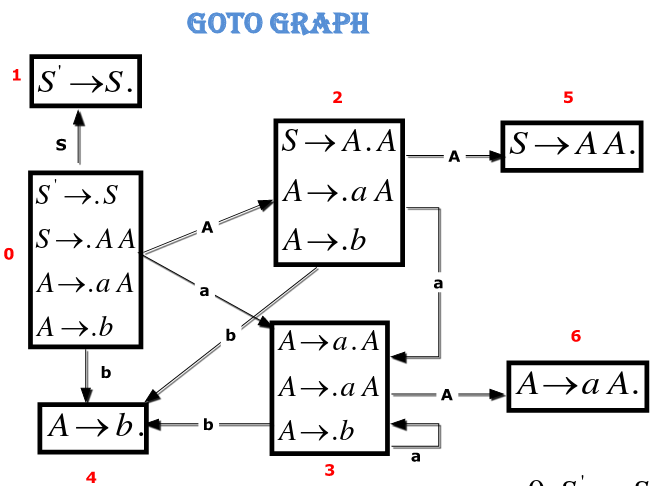
\includegraphics[width=0.8\linewidth]{./assets/goto_graph_example.png}
  \caption{Goto graph}%
  \label{fig:}
\end{figure}

Each edge in the automaton is the goto, and every state is the closure. Using this graph, we can encode it as a parsing table (Fig 2). The goto operations over terminals are equivalent to shift operations. If a state has no outgoing goto operations, we must reduce by the item in that state, over every terminal.

\begin{figure}[htpb]
  \centering
  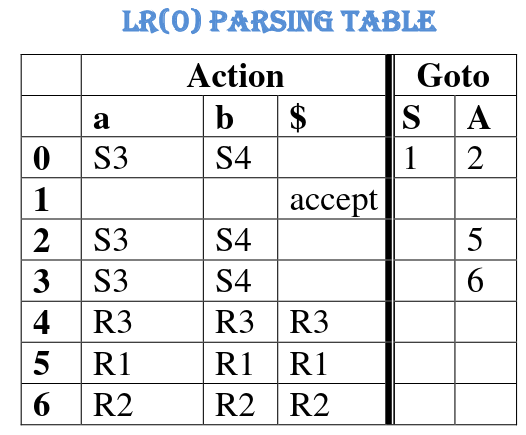
\includegraphics[width=0.6\linewidth]{./assets/lr0_parsing_table_example.png}
  \caption{Parsing Table}%
  \label{fig:./assets}
\end{figure}

The parsing operation of $aabb$ can be seen in Table 1. In the 4th step, we see we pop out $b4$ and push $A6$. How did we decide to move to state 6? This is because of the Goto operation. We checked the preceding state $a3$ and check it's goto over non terminal $A$. This was a transition to state 6.

\begin{table}[htpb]
  \centering
  \caption{Parsing Process}
  \label{tab:label}
  \begin{tabular}{|p{2cm}|p{2cm}|p{10cm}|}
    \hline
    Stack & Input & Action \\
    \hline
    0 & $aabb\$$ & Shift : Push $a$ and state 3 onto the stack \\ 
    0a3 & $abb\$$ & Shift : Push $a$ and state 3 onto the stack \\
    0a3a3 & $bb\$$ & Shift Push $b$ and state 4 onto the stack \\
    0a3a3b4 & $b\$$ & Reduce by $A \rightarrow b$. Pop 2 symbols from the stack and push $A$ and state 6 onto the stack \\
    0a3a3A6 & $b\$$ & Reduce by $A \rightarrow aA$. Pop 4 symbols from the stack and push $A$ and state 6 onto the stack \\
    0a3A6 & $b\$$ & Reduce by $A \rightarrow aA$. Pop 4 symbols from the stack and push $A$ and state 2 onto the stack. \\
    0A2 & $b\$$ & Shift : Push $b$ and state 4 on stack. \\ 
    0A2b4 & \$ & Reduce by $A \rightarrow b$. Pop 2 symbols from the stack and push $A$ and state 5 onto the stack \\
    0A2A5 & \$ & Reduce by $S \rightarrow AA$. Pop 4 symbols from the stack and push state 1 onto the stack. \\
    0S1 & \$ & Accept. \\
    \hline
  \end{tabular}
\end{table}

\subsection{Limitations of the LR(0) Parser}

The primary limitation of the LR(0) parser is that it does not take the lookeahead into account at all - it reduces indiscriminately, regardless of the input token. As such, it only works when states have a single reduce action!

\section{The SLR(1) Parser}

The SLR(1) parser is much like the LR(0) parser, except that the ``reduce'' operations are only written for terminals which are in Follow of the variable whose production is reduced. This way, the SLR parser uses 1 token of lookahead to make it's predictions, which is the reason that we include the 1.

\subsection{Constructing the SLR(1) Parsing Table}

The algorithm for constructing the parsing table is as follows:

\begin{enumerate}
  \item Construct $C = \{I_0,\cdots,I_n\}$ the collection of sets of LR(0) items
  \item If $A \rightarrow \alpha . a\beta$ is in $I_i$ and goto($I_i,a$) = $I_j$, then action[$i,a$] = shift $j$.
  \item If $A \rightarrow \alpha .$ is in $I_i$ then action[$i,a$] = reduce $A \rightarrow \alpha$ for all $a$ in Follow($A$).
  \item If $S' \rightarrow S.$ is in $I_i$, then action[$i,\$$] = accept
  \item If goto($I_i,A$) = $I_j$ then goto[$i,A$] = $j$ for all non terminals $A$
  \item All undefined entries are errors
\end{enumerate}

As we can see, the only difference between this and the LR(0) parser is that the parser will not only reduce in a given state with $A \rightarrow \alpha .$. Instead, it will make smarter decisions based on the follow set.

\subsection{Is it SLR(1)?}

As long as there are no conflicts in the parsing table, the grammar is $SLR(1)$.

\subsection{Limitations of the SLR(1) Parser}

The SLR(1) parser is better, but also does not take into account all the information available. Assume we have a configuration such as $X \rightarrow u .$, we know that this corresponds to having $u$ as a handle at the top of the stack that we can reduce. We do this whenever the input symbol is in Follow($X$). However this may not always be desirable, since elements below $u$ in the stack may preclude $u$ form being a handle for reduction. In other words, SLR only considers the top elements of the stack! We may need to divide the states into parts so that we could consider the different ways in which certain reductions can be carried out.

\section{The Canonical LR(1) Parser}

\subsection{The LR(1) Item}

An LR(1) item has the form $[I,t]$ where $I$ is in LR(0) item and $t$ is a lookahead token. As the dot moves through the right hand side of $I$, token $t$ remains attached to it. When $I$ is of the form $A \rightarrow \alpha . \beta$ and $\beta \neq \epsilon$, the lookahead token has no meaning. However, the LR(1) item $[A \rightarrow \alpha ., t]$ calls for a reduce action if the lookahead is $t$.

\subsection{The Closure Operation}

Closure is done in a different way from LR(0) items. The algorithm is as follows:

\begin{algorithm}[H]
  \SetAlgoLined
  \caption{CLOSURE(I)}
  \While{No more items are added to I} {
    \For{each item $[A \rightarrow \alpha . B \beta,a]$ in $I$}{
      \For{each production $B \rightarrow \gamma$ in G'}{
        \For{each terminal $b$ in First($\beta a$)}{
          add $[B \rightarrow . \gamma, b]$ to set $I$;
        }
      }
    }
  }
  \Return I;
\end{algorithm}

\subsection{The Goto Operation}

For LR(1) items, the algorithm to find the Goto is:

\begin{algorithm}[H]
  \SetAlgoLined
  \caption{GOTO(I)}
  initialize $J$ to be the empty set; \\
  \For{each item $[A \rightarrow \alpha . X \beta, a]$ in $I$}{
    add item $[A \rightarrow \alpha X . \beta, a]$ to set $J$;
  }
  \Return Closure(J);
\end{algorithm}

This is essentially the same as with LR(0) items, but explicitly stating to keep the lookahead token when performing the goto.

\subsection{The CLR(1) Automaton}

Just like before, we can create an automaton representing the operation of the parser. The states are the sets of items and the transitions are the goto over terminals and non-terminals. To get the LR(1) automaton, we can use the algorithm 3. Notice it does exactly the same thing as in an LR(0) parser, but stated in an algorithmic form.

\begin{algorithm}[H]
  \SetAlgoLined
  \caption{items(G')}
  Let $C = CLOSURE(\{[S' \rightarrow .S, \$]\}) \\
  \While{no new sets of items are added to $C$} {
    \For{Each set of items $I$ in $C$}{
      \For{Each grammar symbol $X$}{
        \If{GOTO(I,X) is not empty and not in $C$}{
          add GOTO(I,X) to $C$;
        }
      }
    }
  }
\end{algorithm}

\subsection{The CLR(1) Parsing Table}

Just like before, we have to generate a parsing table to encode the automaton. It is generated as follows:

\begin{enumerate}
  \item Construct $C' = \{I_0,...,I_n\}$, the collection of sets of LR(1) items for $G'$.
  \item State $i$ of the parser is constructed from $I_i$. The parsing action for state $i$ is determined as follows:
    \begin{enumerate}
      \item If $[A \rightarrow \alpha . a \beta, b]$ is in $I_i$ and GOTO($I_i,a$) = $I_j$, then set Action[$i,a$] to shift $j$. Here $a$ is a terminal.
      \item If $[A \rightarrow \alpha ., a]$ is in $I_i$, $A \neq S'$, then set Action[$i,a$] to reduce $A \rightarrow \alpha$.
      \item If $[S' \rightarrow S . , \$]$ is in $I_i$, then set Action[$i,\$$] to accept.
    \end{enumerate}
  \item The goto transitions for state $i$ are constructed for all nonterminals $A$ using the rule: If $GOTO(I_i,A$) = $I_j$, then GOTO[$i,A$] = $j$.
  \item All other entries are error.
  \item The initial state of the parser is the one constructed from the set of items containing $[S' \rightarrow .S,\$]$
\end{enumerate}

\subsection{Is a Language CLR(1)?}

A language is CLR(1) if and only if the parsing table does not have repeated entries.

\section{The LALR parser}

\subsection{Why Do We Need It?}

Generally, LALR parsers are used over CLR parsers. This is because CLR parsers would have thousands of states for a grammar that an LALR parser could parse with hundreds of states. It is hence more economical to use these in practice. LALR reduces the number of states by merging similiar sets. For instance, if we have two sets:
\[[A \rightarrow b ., a/b]\]
\[[A \rightarrow b ., \$]\]
We could merge them to create
\[[A \rightarrow b . , a/b/\$]\]

Those two sets are said to share a common \textbf{core}.

\subsection{Parse Table Construction}

The construction of a parse table for LALR works as follows:

\begin{enumerate}
  \item Construct $C = \{I_0,I_1,\cdots,I_n\}$, the collection of sets of LR(1) items
  \item Find all the sets sharing the same cores, and merge them into their union.
  \item Let $C' = \{J_0,J_1,\cdots,J_m\}$ be the resulting sets. The parsing actions for each of these states are the same as in CLR(1).
  \item The Goto table is constructed as follows. If $J$ is the union of one or more sets of LR(1) items, that is $J = I_1 \cup I_2 \cup \cdots \cup I_k$, then the cores of GOTO($I_1,X$), GOTO($I_2,X$), ... , GOTO($I_k,X$) are the same, since $I_1,I_2,...,I_k$ all have the same core. Let $K$ be the union of all sets of items having the same core as GOTO($I_1,X$). Then GOTO($J,X$) = $K$.
\end{enumerate}

The meaning of (4) is that we can just directly merge the rows of the CLR(1) parsing tables of $I_1,...,I_k$ to get the LALR parsing table. In case there is an overlap, that overlap would be a merged set present in $C'$.

\subsection{Relative Power}

The relative power of LALR(1) is actually less than CLR(1), since it merges some states that could have earlier contained some contextual information. When talking about parsers,
\[LR(0) \subset SLR \subset LALR(1) \subset CLR(1)\]
The LL(1) parser has no direct relation to them - however, $LL(1) \subset LR(1)$. This relation is in fact true for all $k$ in LL(k) and LR(k).

\chapter{Semantic Analysis}

\section{Introduction}

A parser cannot catch all the program errors. Some language features cannot be modelled using context free grammars. For instance, a parser cannot find whether an identifier has been declared before use, and cannot check scoping rules.

The semantic analyzer takes the generated parse tree as input and gives an unambiguous program representation in the form of the disambiguated parse tree.

Some semantic errors could be:

\begin{itemize}
  \item Type errors
  \item Use of undeclared variables
  \item An identifier may refer to different variables in different parts of the program
  \item An identifier may be usable in one part of the program but not another.
\end{itemize}

\section{Attribute Grammar Framework}

The attribute grammar framework is the generalization of CFGs where each grammar symbol has an associated set of attributes. The semantic attributes are computed according to some semantic rules.

The attribute grammar framework is generally notated by the \textbf{syntax directed definition}. Attributes are associated with grammar symvols and rules are associated with productions. If $X$ is a symbol and $a$ is one of its attributes, then we write $X.a$ to denote the value of $a$ at a particular parse tree node labeled $X$.

Non terminals can have two types of attributes:

\begin{itemize}
  \item A \textbf{synthesizes attribute} for a non terminal $A$ at a parse tree node $N$ is defined by a semantic rule associated with the production at $N$. Note that the production must have $A$ as it's head.
  \item An \textbf{inherited attribute} for a non terminal $B$ at a parse tree node $N$ is defined by a semantic rule associated with the production at the parent of $N$. The production must have $B$ as a symbol in it's body.
\end{itemize}

An SDD that uses only synthesized attributes is said to be an S-attributed definition.

Let us consider the following example grammar for arithmetic expressions:
\[L \rightarrow E\]
\[E \rightarrow E + T\]
\[E \rightarrow T\]
\[T \rightarrow T \times F\]
\[T \rightarrow F\]
\[F \rightarrow (E)\]
\[F \rightarrow id\]

The associated S-attributed SDD, in order will be:
\[Print(E.val)\]
\[E.val = E.val + T.val\]
\[E.val = T.val\]
\[T.val = T.val \times F.val\]
\[T.val = F.val\]
\[F \rightarrow E.val\]
\[F.val \rightarrow id.lexval\]

\section{Dependency Graphs}

To evaluate an SDD, we generally use \textbf{dependency graphs}. A dependency graph shows the interdependencies among the attributes of the various nodes of a parse tree. If an attribute $b$ depends on an attribute $c$, we add an edge $c \rightarrow b$ in the dependency graph. If $c \rightarrow b$, then we need for use the semantic rule of $c$ first, and then the semantic rule for $b$.

As an example, let us consider the following grammar:
\[D \rightarrow TL\]
\[T \rightarrow real\]
\[T \rightarrow int\]
\[L \rightarrow L_1,id\]
\[L \rightarrow id\]

The associated SDD (in order) will be:
\[L.in = T.type\]
\[T.type = real\]
\[T.type = int\]
\[L_1.in = L.in\]
\[addtype(id.entry,L.in)\]

Here, the first rule is an inherited attribute. We can always write a grammar with only synthesized attributes, but including inherited attributes makes it simpler.

Then, the parse tree and associated dependence graph (shown in green) for an input \texttt{real x,y,z} will be as seen in Fig 1.

\begin{figure}[htpb]
  \centering
  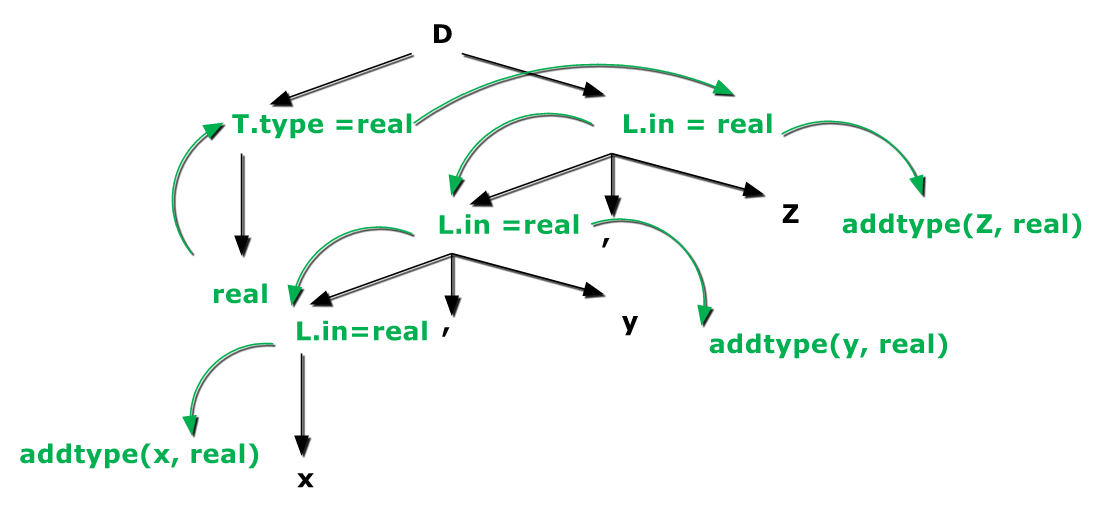
\includegraphics[width=0.8\linewidth]{./assets/dep_graph_eg.png}
  \caption{Dependency graph for the given grammar}%
  \label{fig:}
\end{figure}

\section{Abstract Syntax Tree}

AST is condensed form of parse tree. Chains of single productions can be collapsed, and operators move to the parent nodes. An example can be seen in Fig 2.

\begin{figure}[htpb]
  \centering
  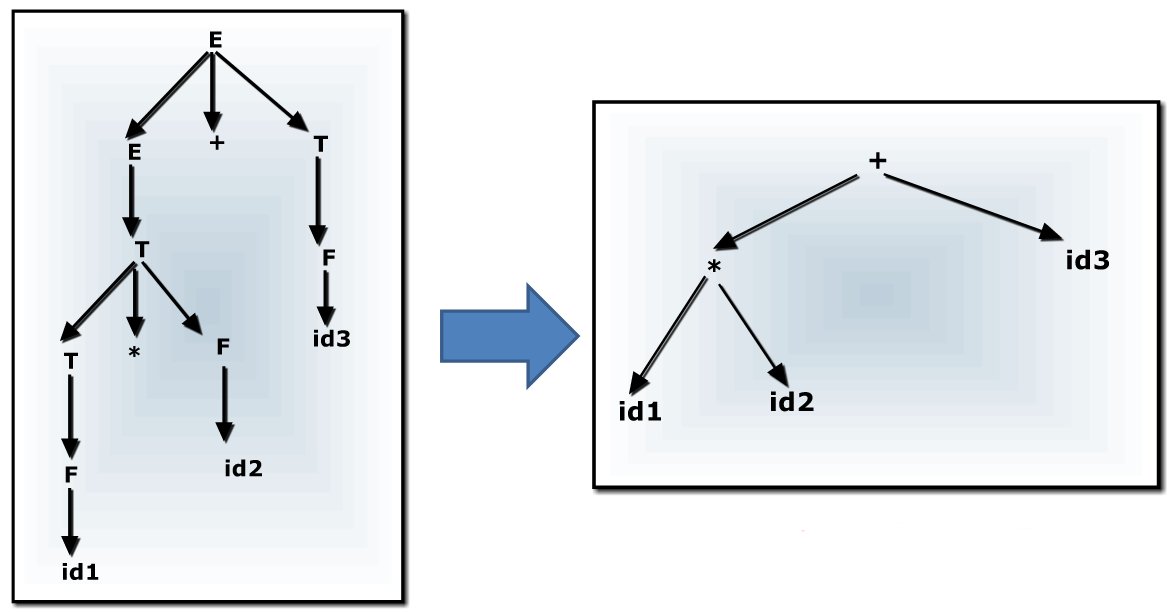
\includegraphics[width=0.8\linewidth]{assets/ast_eg.png}
  \caption{Abstract Syntax Tree}%
  \label{fig:}
\end{figure}

Each node can be represented as a record. In the above grammar, the operators can be represented by a record with a field for the operator type and remaining fields as pointers to operands. Every identifier can be a record with the label id and another pointer to the symbol table. Numbers can be records with a field for the label num and another to keep the number's value.

Consider the grammar:
\[E \rightarrow E_1 + T\]
\[E \rightarrow T\]
\[T \rightarrow T_1 * F\]
\[T \rightarrow F\]
\[F \rightarrow (E)\]
\[F \rightarrow id\]
\[F \rightarrow num\]

The respective operations to build the AST would be:
\[E.ptr = mknode(+,E_1.ptr,T.ptr)\]
\[E.ptr = T.ptr\]
\[T.ptr = mknode(*,T_1.ptr,F.ptr)\]
\[T.ptr = F.ptr\]
\[F.ptr = E.ptr\]
\[F.ptr = mkleaf(id,entry.id)\]
\[F.ptr = mkleaf(num,val)\]

We use $mkleaf$ to create leaf nodes and $mknode$ to make internal nodes.

\section{L Attributed Definitions}

L attributed definitions contain both synthesized and inherited attributes. A syntax directed definition is L attributed if each inherited attribute of $X_j$ in a production:
\[A \rightarrow X_1 \cdots X_j \cdots X_n\]
depends only on
\begin{itemize}
  \item The attributes of the symbols to the left of $X_j$
    \irem The inherited attributes of $X_j$
\end{itemize}

$A \rightarrow BC \{B.S = A.S\}$ is an example of an L-attributed definition.

In an L-attributed definition, attributes can be evaluated in depth first order, which is natural for both top down and bottom up parsing.

The following SDD is a L-attributed definition
\[A \rightarro LM\]
\[L.i = f_1(A.i)\]
\[M.i = f_2(L.s)\]
\[A.s = f_3(M.s)\]

The following SDD is not a L-attributed definition
\[A \rightarrow QR\]
\[R.i = f_4(A.i)\]
\[Q.i = f_5(R.s)\]
\[A.s = f_6(Q.s)\]

(why?)

\section{Translation Scheme}



\end{document}
